\chapter{Background}
\label{chap:Two}

\section{The Auto-Formalization Challenge}
Auto-formalization is defined as the automated process of translating informal, human-readable mathematical language—such as that found in standard academic textbooks and research papers—into a strict, machine-verifiable representation \cite{autoform_survey, proof_systems}. Achieving this translation bridge is notoriously difficult. Natural language math relies heavily on context and implicit assumptions ("let $X$ be a space," where the topology is implicitly understood). Formal systems, however, lack intuition and demand explicitly declared types, universes, and axioms \cite{formal_history}.

Historically, this translation has been a painstakingly manual and labor-intensive task, effectively restricting formal mathematics to a niche community of specialized logicians \cite{formal_history}. However, the rapid advancement and wide availability of Large Language Models (LLMs) have provided a potential solution. These probabilistic models have shown remarkable capabilities in parsing syntax, semantic decomposition, and "translating" abstract concepts across different languages, including programming code \cite{llm_math, llm_codegen}. 

\begin{figure}[h]
\centering
\begin{center}
    \IfFileExists{img/rosetta_stone.jpg}{
        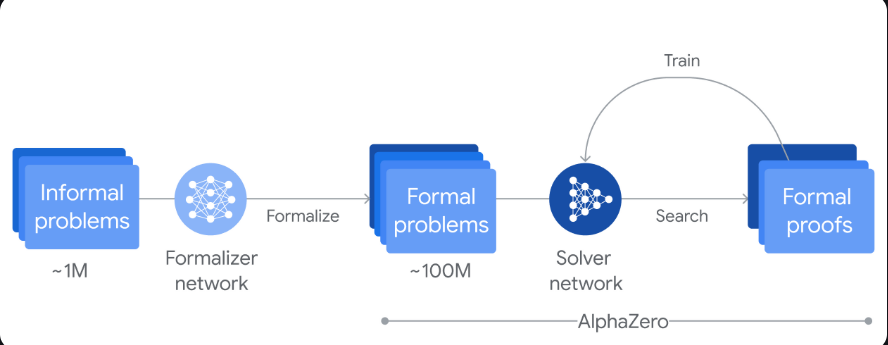
\includegraphics[width=0.7\textwidth]{img/rosetta_stone.jpg}
    }{
        \fbox{\begin{minipage}[c][4cm][c]{0.7\textwidth}\centering Image: Visual Comparison of Informal English vs. Formal Code (Placeholder)\end{minipage}}
    }
\end{center}
\caption{The ``Rosetta Stone'' Concept: Bridging Natural Language and Formal Logic. The English text acts as the conceptual layer, while the formal code acts as the verifiable foundation.}
\label{fig:rosetta_concept}
\end{figure}

\section{Lean 4: A Modern Theorem Prover}
Unlike standard programming languages, \texttt{Lean 4} operates both as a functional programming language and as an immensely powerful interactive theorem prover based on the Calculus of Inductive Constructions (a variant of dependent type theory) \cite{lean4_doc}. 
\begin{itemize}
    \item \textbf{Dependent Types:} In Lean, types can depend on values (e.g., an array of length $n$). This allows mathematicians to encode complex logical propositions directly into the type framework itself.
    \item \textbf{Tactics Engine:} Lean uses a sophisticated "tactics" engine (utilizing commands like \texttt{rw}, \texttt{simp}, \texttt{induction}, and \texttt{apply}) to manipulate logical states, breaking down a complex mathematical goal until it matches known axioms \cite{lean_tactics}.
    \item \textbf{Mathlib4:} The Lean ecosystem is uniquely powered by \texttt{Mathlib}, a massive, community-driven, crowdsourced library containing tens of thousands of formalized theorems across algebra, topology, and calculus \cite{mathlib, lean4_doc}. It provides the necessary foundation for the ``Truth Scanner'' pipeline.
\end{itemize}

\section{Neuro-Symbolic AI Pipelines}
This thesis utilizes a neuro-symbolic approach to solve the auto-formalization challenge, a technique highly inspired by recent high-profile research like DeepMind's AlphaProof \cite{alphaproof2024, neural_formal}. Pure neuro-models (like ChatGPT) are excellent semantic engines but struggle with strict rule adherence, frequently leading to "hallucinations"—convincingly stated but mathematically impossible conclusions \cite{llm_hallucination, proof_systems}.

By building a neuro-symbolic pipeline, we segment responsibilities: 
\begin{enumerate}
    \item \textbf{The Neuro Layer (LLM):} Handles the creative translation and contextual interpretation of the ambiguous English text.
    \item \textbf{The Symbolic Layer (Lean 4):} Provides the rigorous, uncompromising cryptographic verification of the translated logic \cite{llm_math, symbolic_ai}.
\end{enumerate}
This dual-engine architecture guarantees that if an auto-generated formalization successfully compiles in the symbolic layer, it is definitively true, completely eradicating the issue of AI hallucinations.

\section{Manual Formalization Example: The Ground Truth}
To train, evaluate, and benchmark the LLM capabilities within our automated pipeline, it is necessary to first manually formalize a core library of mathematical definitions from Rosen's textbook \cite{rosen2019}. This manually curated code serves as our absolute "Ground Truth". 

For instance, the definitions of basic Set Theory and Logic—such as logical implication, set intersection, subset relations, and function injectivity—have been successfully transcribed into functional Lean 4 code within our \texttt{Definitions.lean} module. Formalizing even elementary concepts like a subset requires strict syntax, explicit variable typing (such as \texttt{variable \{$\alpha$ : Type\}}), and logic quantifiers that are entirely abstracted away in natural English texts. Understanding this structural gap is essential for building the auto-prompts required for the LLM pipeline discussed in the subsequent chapters.